\documentclass[11pt]{article}

\usepackage{geometry}
 \geometry{
 a4paper,
% total={210mm,297mm}
% }
 left=17mm,
 right=23mm,
 top=20mm, 
 bottom=20mm,
 }
\usepackage{url}
\usepackage{rotating}
\usepackage{natbib}
\usepackage{placeins}
\usepackage{longtable}
\usepackage[latin1]{inputenc}
\usepackage{multirow}
\usepackage{hyperref}
%\usepackage{showframe}
\usepackage{pdflscape}
%\usepackage{pbox}
\usepackage{xcolor}
\usepackage{amsmath}
\usepackage{rotating}
\usepackage{multicol}
\usepackage{caption}
\usepackage{subfigure}



\usepackage{pdflscape}

\usepackage{listings}

\lstset{
  basicstyle=\ttfamily, 
  basewidth=0.5em,                 %the default setting of listings with "fixed columns" has a space 0.6em wide, 
                                   %while the characters in Computer Modern Typewriter are 0.5em wide.
                                   %http://tex.stackexchange.com/questions/179071/spacing-looks-wrong-in-listings-when-using-fixed-columns
  backgroundcolor=\color{gray!10},
  keywordstyle=\color{green!40!black},
  columns=fixed,
  language=R,                     % the language of the code
  basicstyle=\footnotesize,       % the size of the fonts that are used for the code
  numbers=left,                   % where to put the line-numbers
  numberstyle=\tiny\color{gray},  % the style that is used for the line-numbers
  stepnumber=1,                   % the step between two line-numbers. If it's 1, each line
                                  % will be numbered
  numbersep=5pt,                  % how far the line-numbers are from the code
  showspaces=false,               % show spaces adding particular underscores
  showstringspaces=false,         % underline spaces within strings
  showtabs=false,                 % show tabs within strings adding particular underscores
  frame=single,                   % adds a frame around the code
  rulecolor=\color{black},        % if not set, the frame-color may be changed on line-breaks within not-black text (e.g. commens (green here))
  tabsize=2,                      % sets default tabsize to 2 spaces
  captionpos=b,                   % sets the caption-position to bottom
  breaklines=true,                % sets automatic line breaking
  breakatwhitespace=false,        % sets if automatic breaks should only happen at whitespace
  title=\lstname,                 % show the filename of files included with \lstinputlisting;
                                  % also try caption instead of title
  keywordstyle=\color{blue},      % keyword style
  commentstyle=\color{green},   % comment style
  stringstyle=\color{red},      % string literal style
  escapeinside={\%*}{*)},         % if you want to add a comment within your code
  morekeywords={*,...}            % if you want to add more keywords to the set
} 

\usepackage{graphicx}
\usepackage{gensymb}
\usepackage{nag}   %It warns the user about the usage of old packages or commands (for example, using \it, \tt, etc.)
\usepackage{fixltx2e}
%fixltx2e package. It fixes some 'mistakes' in Latex. From the description:
%        ensure one-column floats don't get ahead of two-column floats;
%        correct page headers in twocolumn documents;
%        stop spaces disappearing in moving arguments;
%        allowing \fnysmbol to use text symbols;
%        allow the first word after a float to hyphenate;
%        \emph can produce caps/small caps text;
\usepackage{booktabs}
% \centering instead of \begin{center} \end{center} to center things inside tables/figures etc. \centering doesn't add any additional vertical space.
\usepackage{microtype}  %for small-scale typographic enhancements (character protrusion, font expansion, letter-spacing).
\usepackage{fancyvrb}   %get precise control in verbatim listings.
%\usepackage{siunitx} To typeset units
\usepackage{numprint} %format numbers nicely 
%~, the non-breakable space.

\parindent=0pt
\parskip=8pt
\setlength\itemsep{0em}

%\sloppy
%\SweaveOpts{echo=FALSE,prefix.string=script18/plot}
\renewcommand{\textfraction}{0.0}

\let\oldmarginpar\marginpar
\renewcommand\marginpar[1]{\-\oldmarginpar[\raggedleft\footnotesize #1]%
{\raggedright\footnotesize #1}}

\newcommand{\supp}{\mathop{\mathrm{supp}}}

\newcommand{\cursedforest}{{\sc CursedForest}}
\newcommand{\mtry}{{\texttt mtry}}
\newcommand{\ntree}{{\texttt ntree}}


\newsavebox\ltmcbox

\title{\cursedforest\ - A Random Forest Implementation for ``Big'' and ``Wide'' Data \\
Supplementary Information}
\author{}
\date{}



\begin{document}
%\setkeys{Gin}{width=8cm}
\setkeys{Gin}{height=8cm,width=0.9\columnwidth}
\maketitle
%%\tableofcontents
%% ## \begin{landscape}
%% ##   \small
%% ## \end{landscape}


%% \begin{lstlisting}
%% \end{lstlisting}




\section{supplementary Information for Section 4.1}

\begin{sidewaystable}[!ht]
\begin{minipage}{\textwidth}
%\begin{adjustwidth}{-2.25in}{0in} % Comment out/remove adjustwidth environment if table fits in text column.
\centering
\caption{
{\bf Performance comparison between the different machine learning algorithms.}}
\begin{tabular}{|l|l|l|l|l|l|p{1cm}|}
\hline
\bf{Genome \%}                      & \bf{Method} & \bf{Error (ARI)} & \bf{Runtime} & \bf{Memory/Node} \\
\hline

\multirow{3}{*}{phase1\_chr22: 1,092 x 490,036} & \cursedforest & 0.04  & 1 min 50 seconds  &  \\ %110 %\cursedforest\ & 0.077 (XX) &                  &                                                                   \\
                                                & RF - Spark ML  &  0.05           &           7 mins 44 seconds        &  \\  %464  %&            &                  &                                                                   \\
                                                & randomForest - R         & 0.05       & 24 mins           & 18GB\footnote{using the \texttt{parallel} packages with 10 nodes} \\ %1440
                                                & ranger - R      & 0.06       & 1 min 10 seconds & 16GB  (one processor)                                             \\ %70
                                                & ranger - c++     & 0.06       & 7 mins           & --nthreads 20                                                    \\  %420
                                                & H2O           & 0.06       & 5 hours         & 600GB \footnote{java -Xmx600g -jar h2o.jar,   h2o.init(nthreads=20)} \\ %18000

 \hline
\multirow{3}{*}{phase3\_chr22: 2,504 x 1,103,548}   & \cursedforest & 0.06 & 4 mins 2 seconds & \\  %240 &               &            &                  &                                                                \\
						  & RF - Spark ML   & 0.06 & 37 mins 19 seconds  & \\  %2239
                                                    & randomForest - R        & NA         & NA               & NA\footnote{long vectors ($> 2^31-1$)  are not supported in the .Fortran interface} \\ %OK
                                                    & ranger - R    & 0.06       & 18 mins        & 21GB (one processor) \\ %1080
                                                    & ranger - c++ & 0.05  & 1 hour 3 min &   \\  %3780
			                           & H2O           & 0.05       & 16 hours         & 600GB \footnote{java -Xmx600g -jar h2o.jar,   h2o.init(nthreads=20)} \\  %57600
\hline
\multirow{3}{*}{phase3\_chr1: 2,504 x 6,450,364}    & \cursedforest & 0.04  & 19 mins 19 seconds &        \\ %1159   \cursedforest\ & 0.06 & 1hr 58min        & 4GB \\
                                                    & RF - Spark ML  &  0.04       & 8 hours 29 mins   &     \\ % 3403 0.06       & 8hr 29min        & 8GB \\
  %                                                  & LR - Spark ML  &            & 2hr 6min         & 8GB \\
                                                   & ranger - R      & 0.05       & 1 hour 42 mins          & num.threads=10  \\ %6120
                                                   & ranger - c++ & 0.04 & 5 hours 27 mins &  \\ %19620
                                                    &H2O & NA & NA &   \\
\hline
\multirow{3}{*}{phase3\_chr1-3: 2,504 x 19,328,051} & \cursedforest & 0.02  & 56 mins 43 seconds     &        \\ %3403%& 0.04 & 4hr 0min                                             & 4GB \\
                                                    & RF - Spark ML  &  NA           &  NA                                                     & \\ %OK
  %                                                  & LR - Spark ML  &            & 14hr 48min                                           & 8GB \\
  						 & ranger - R      & 0.03      &    3 hours 58 mins  &   \\ %14280
						& ranger - c++ & 0.04 & 8 hours 54 mins &  \\ %32040
\hline
\multirow{4}{*}{phase3\_chr1-22: 2,504 x 81,047,467} & \cursedforest\ & 0.01  & 3 hours 16min & \\% \\ %11760 %& 0.04 & 7hr 14min & 8GB \\
%& kmeans - Spark ML  & 0.18      & 30hr 44min    & 24GB \\ 
										& ranger - R       &        NA     &        NA   & \\
										& ranger - c++       &        NA     &        NA     &            80 CPU -- runs out of memory (12.8GB per CPU) \\
										& ranger - c++       &        NA     &        NA     &            160 CPU -- runs out of time at 20 hours \\
\hline
\end{tabular}
\begin{flushleft} 
Comparison of different various machine learning libraries on different subsets of variant data 
from the 1000 Genomes Project.
Each random forest model consists of 50 trees.
\end{flushleft}
\label{table1}
%\end{adjustwidth}
\end{minipage}
\end{sidewaystable}

\clearpage
\newpage

\section{supplementary Information for Section 4.2}

\begin{figure}[tbhp]
    \caption{\textbf{Rank of literature assigned BMD genes}}
    \label{figure:knowngeneranks}
    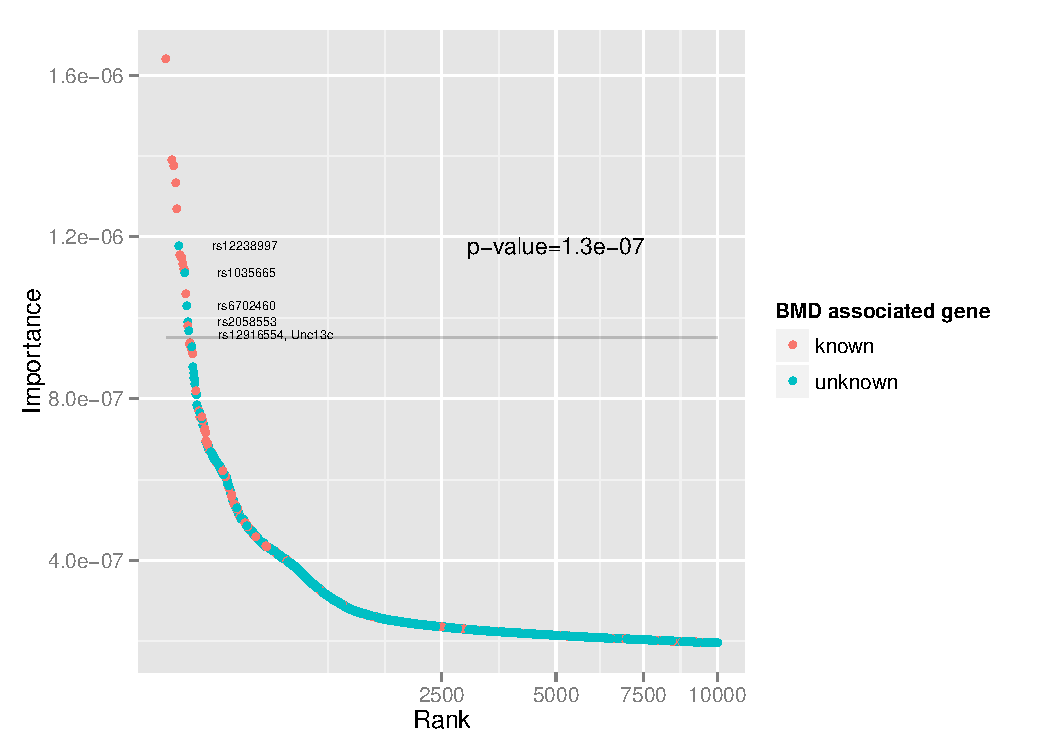
\includegraphics{./figs/BMDTop10K.pdf}
    \begin{flushleft}
      The figure shows the top 10,000 features by their rank and Gini impurity score (Importance). The line denotes the top 30 features which contains six novel loci. 
     \end{flushleft}
\end{figure}




\begin{figure}[tbhp]
    \caption{\textbf{Zoomplot in order of importance}}
    \label{figure:knowngeneranks}
    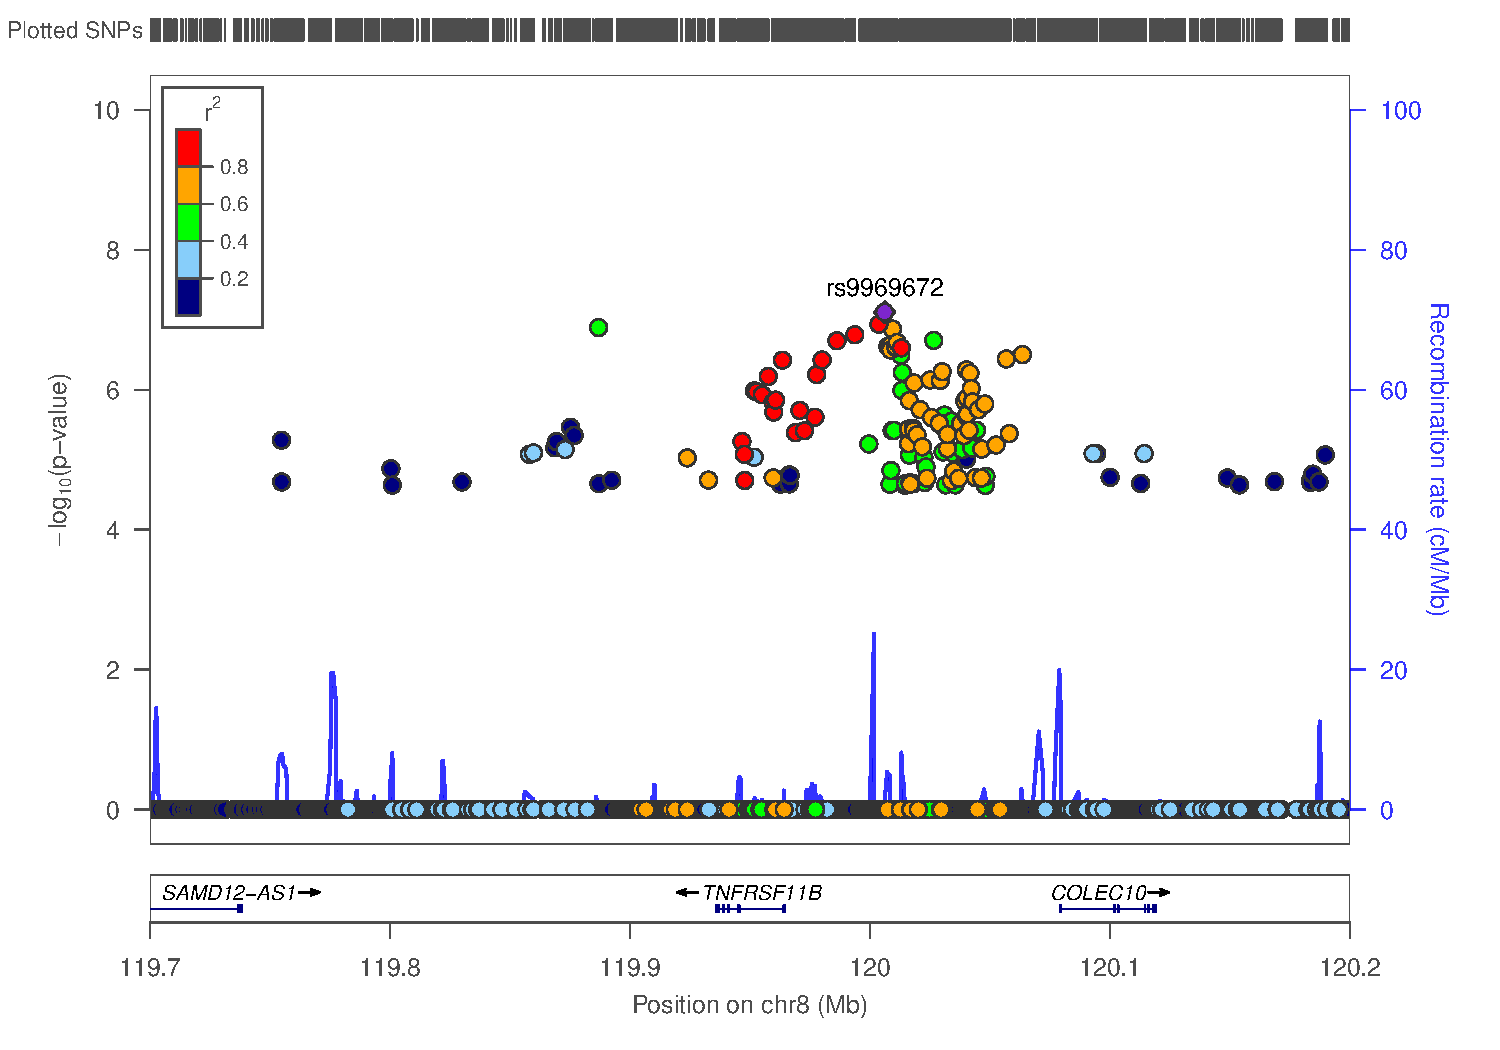
\includegraphics{./figs/new_10k_TNFRSF11B.pdf}
     \includegraphics{./figs/new_10k_CTNNB1.pdf}
    \begin{flushleft}
     \end{flushleft}
\end{figure}


\begin{figure}[tbhp]
    \caption{\textbf{Zoomplot in order of importance}}
    \label{figure:knowngeneranks}
      \includegraphics{./figs/new_10k_ZBTB40.pdf}
        \includegraphics{./figs/new_10k_IBSP.pdf}
    \begin{flushleft}
     \end{flushleft}
\end{figure}


\begin{figure}[tbhp]
    \caption{\textbf{Manhattan plot of PRODH and LINC01006}}
    \label{figure:knowngeneranks}
        \includegraphics{./figs/BMDTopWholeGenome_22.pdf}
      \includegraphics{./figs/BMDTopWholeGenome_7.pdf}
    \begin{flushleft}
     \end{flushleft}
\end{figure}


\bibliographystyle{apalike}

%\bibliography{/home/dun280/Dropbox/TeX/bibliography/screening_compliance.bib}
\bibliography{/home/dun280/Dropbox/TeX/bibliography/ripley.bib}
\end{document}





\begin{sidewaystable}[!ht]
\begin{minipage}{\textwidth}
%\begin{adjustwidth}{-2.25in}{0in} % Comment out/remove adjustwidth environment if table fits in text column.
\centering
\caption{
{\bf Performance comparison between the different machine learning algorithms.}}
\begin{tabular}{|l|l|l|l|l|l|p{1cm}|}
\hline
\bf{Genome \%}                      & \bf{Method} & \bf{Error}  & \bf{Runtime} & \bf{Memory/Node} \\
\hline

\multirow{3}{*}{phase1\_chr22: 1,092 x 490,036} & \cursedforest\ & 0.077  &                  &                                                                   \\
                                                & Spark ML  &            &                  &                                                                   \\
                                                & RF - R         & 0.05       & 24 min           & 18GB\footnote{using the \texttt{parallel} packages with 10 nodes} \\
                                                & ranger - R      & 0.06       & 1 min 10 seconds & 16GB  (one processor)                                             \\
                                                & ranger - c++     & 0.06       & 7 mins           & --nthreads 20                                                     \\

 \hline
\multirow{3}{*}{phase3\_chr22: 2,504 x 1,103,548}   &               &            &                  &                                                                \\
                                                    & RF - R        & NA         & NA               & NA\footnote{long vectors ($> 2^31-1$)  are not supported in the .Fortran interface} \\
                                                    & H2O           & 0.05       & 16 hours         & 600GB \footnote{java -Xmx600g -jar h2o.jar,   h2o.init(nthreads=20)} \\
                                                    & ranger - R    & 0.06       & 4 1/2 mins       & 21GB (one processor) \\
\hline
\multirow{3}{*}{phase3\_chr1: 2,504 x 6,450,364}    & \cursedforest\ & 0.063  & 1hr 58min        & 4GB \\
                                                    & Spark ML  & 0.94       & 8hr 29min        & 8GB \\
                                                    & ranger - R      &  0.05       & 28 mins          & num.threads=10\footnote{don't
                                                                                                      know how to get the memory
                                                                                                      used,   This was done on dpas-03} \\
\hline
\multirow{3}{*}{phase3\_chr1-3: 2,504 x 19,328,051} & \cursedforest\ & 0.046  & 4hr 0min                                             & 4GB \\
                                                    & RF - Spark ML  &            &                                                      & \\
                                                    & ranger - R      & 0.03      & 58 mins\footnote{ but took 6 hours to load the
                                                                                   data}
                                                                                                                                         &
                                                                                                                                           909GB\footnote{I
                                                                                                                                           think
                                                                                                                                           this
                                                                                                                                           is
                                                                                                                                           total
                                                                                                                                           memory. The
                                                                                                                                           job
                                                                                                                                           was
                                                                                                                                           run
                                                                                                                                           with
                                                                                                                                                   ntasks-per-node=160
                                                                                                                                           cores-per-socket=10
                                                                                                                                           on
                                                                                                                                           ruby
                                                                                                                                           }  \\
& ranger - R        &             0.973     &      03:58           &       pearcey --cpus-per-task=15 --mem 1600gb   906GB \\
\hline

\multirow{4}{*}{phase3\_chr1-22: 2,504 x 81,047,467} & \cursedforest\ & XX (0.96) & 7hr 14min & 8GB \\
& Spark ML & - & - & - \\
& ranger (C++)       &        NA     &        NA     &            80 CPU -- runs out of memory (12.8GB per CPU) \\
& ranger (C++)       &        NA     &        NA     &            160
                                                        CPU -- runs
                                                        out of time at
                                                        20 hours \\
\hline
\end{tabular}
\begin{flushleft} 
Comparison of different various machine learning libraries on different subsets of variant data 
from the 1000 Genomes Project.
Each random forest model consists of 50 trees.
\end{flushleft}
\label{table1}
%\end{adjustwidth}
\end{minipage}
\end{sidewaystable}






% \begin{tabular}{|p{1.2cm}|p{1cm}|p{1.5cm}+l|l|p{1.8cm}|p{1.5cm}|}
% \hline
% %\multicolumn{4}{|l|}{\bf Heading1} & \multicolumn{4}{|l|}{\bf Heading2}\\ \hline
% \bf{Data- set} & \bf{Samp- les} & \bf{Feat- ures}  & \bf{Method} & \bf{Error (ARI)} & \bf{Runtime} & \bf{Memory/ Node} \\
% \hline
% %\multirow{3}{*}{phase1\_chr22: 1,092 x 490,036} & CursedForest & 0.077 (XX)  &  &  \\
% phase1 chr22 &1,092 & 490,036 & CursedForest & 0.077 (XX)  & 9min 16sec & 1GB\footnote{\label{note10}10 nodes} \\
% &&& RF - Spark ML & 0.069 (0.89) & 14min 13sec & 1GB\footref{note10}  \\
% &&& RF - R &  0.05  & 24min  & 18GB\footref{note1}\footnote{using the \texttt{parallel} packages}\\
% &&& ranger -R &         0.05 &        1min 10sec  &          16GB  (one processor) \\
%  \hline
% phase3 chr22 & 2,504 & 1,103,548 &  &  &  &  \\
% &&& CursedForest & 0.053 & 9 min 8 sec & 2GB\footnote{\label{note20}20 nodes}\\
% &&& RF - Spark ML & 0.058 (0.92) & 1hr 1min & 2GB\footref{note20} \\
% &&& RF - R & NA  & NA & NA\footnote{long vectors ($> 2^31-1$)  are not supported in the .Fortran interface}\\
% &&&  H2O   &        0.05 &     16 hours       &   600GB \footnote{java -Xmx600g -jar h2o.jar,   h2o.init(nthreads=20)} \\
% \hline
% phase3 chr1 & 2,504 & 6,450,364 & CursedForest & 0.063 (XX) & 1hr 58min & 4GB \\
% &&& RF - Spark ML & (0.94) & 8hr 29min & 8GB \\
% &&& LR - Spark ML&  & 2hr 6min & 8GB\\ 
% &&& ranger  R   &  0.06   &     28 mins  &            num.threads = 10\footnote{don't know how to get the memory used, This
%   was done on dpas-03} \\ 
% \hline
% phase3 chr1-3 & 2,504 & 19,328,051  & CursedForest & 0.046 (XX) & 4hr 0min & 4GB\\
% &&& RF - Spark ML & - & -  & -\\
% &&& LR - Spark ML & & 14hr 48min & 8GB \\ 
% &&& ranger  R   &  0.05   &     58 mins\footnote{ but took 6 hours to load the data}  &      909GB\footnote{I think this is total memory. The job was run with
%   ntasks-per-node=160 cores-per-socket=10 on ruby }  \\ 
% \hline
% phase3 chr1-22 & 2,504 & 81,047,467 & CursedForest & XX (0.96) & 7hr 14min & 8GB \\ 
% &&& RF - Spark ML & - & - & - \\
% &&& LR - Spark ML & - & - & - \\ 
% %&&& kmeans - Spark ML & - (0.82) & 30hr 44min & 24GB \\ 
% \hline
